\thispagestyle{empty}

\begin{center}
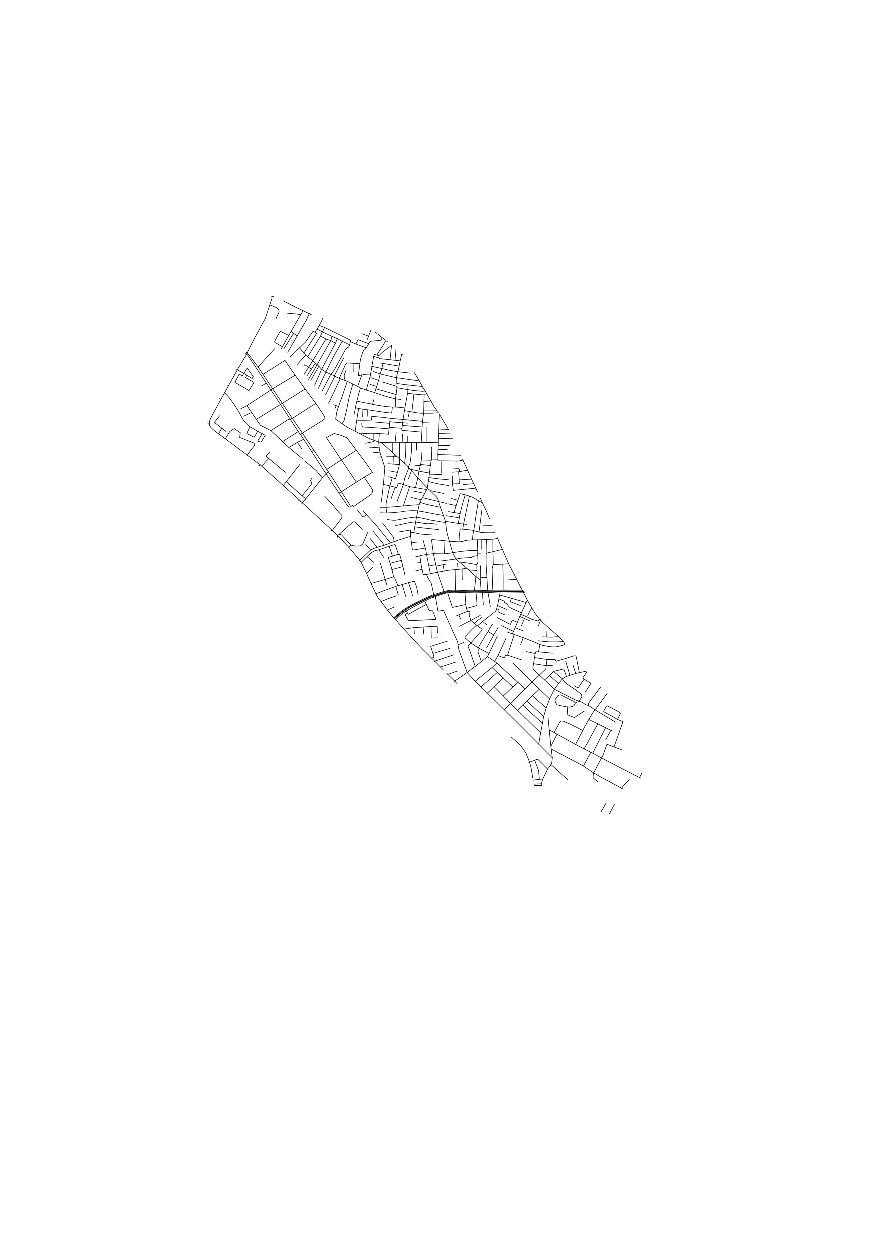
\includegraphics{maps/ejipura.pdf}

 \textit{``It is a handsome city, but distractingly regular. After walking about it for an hour or two, I felt that I would have given the world for a crooked street."} \\ \vspace{5pt}
    \small - Charles Dickens
\end{center}

\newpage
\section*{Acknowledgments}
It took a small village to get this book done. I would like to express my profound gratitude to my friends and family, whose unwavering support, encouragement, and occasional interventions were instrumental in keeping me sane during this academic ordeal.

Anshu, for holding down the fort in 301 Danville while I disappeared for days and for the copyediting I know he will do on this book.

My mother and father, for their constant interest and support which motivated me to keep going. Few parents set up Google Meets to discuss work.

Rhea, who set the bar with her way of working, and pushed me to do this in half the time I would have taken otherwise.

Sahana, without whose help I would not have kept up in class and for letting me copy her notes all the time.

Lakshmi, for all the one-on-ones and pushing me to get out of my comfort zone.

Adhavan and Vivek, who accompanied me on walks to Ejipura and for being excellent collaborators every step of the way.

Abhishek, who accompanied me for street audits and helped me immensely with interviews.

Herry Gulabani, for introducing me to Ejipura and helping shape my research questions.

IKEA Nagasandra, whose endless supply of coffee and food kept me fueled and for not kicking me out.

Santosh, Kaka and all the Sundaram crew, for everything they've done for me over the last four years.

Arvind Venkatadri, who introduced me to R and Rmarkdown four years ago and challenged me to write my thesis with it. Here you go.

\setlength{\abovedisplayskip}{-5pt}
\setlength{\abovedisplayshortskip}{-5pt}
